\documentclass[11pt,twocolumn]{article}
\usepackage[hyperref]{acl2020}
\usepackage{geometry}
%\usepackage{showframe} %This line can be used to clearly show the new margins
\newgeometry{vmargin={20mm}, hmargin={20mm,25mm}}   % set the margins\usepackage{graphicx}
\usepackage{floatflt}
%\usepackage{fdsymbol}
%\usepackage{tabularx,supertabular}
%\usepackage{apacite}
%\usepackage[round]{natbib}
%\usepackage{wasysym}
%\usepackage{draftcopy}
\aclfinalcopy
\pagestyle{plain}
\usepackage{times}
\usepackage{latexsym}
\usepackage{microtype}
\usepackage{caption}
\usepackage{xcolor}
%\usepackage[firsttwo,light]{draftcopy}
%\usepackage{setspace}
%\doublespacing
%\interlinepenalty=10000
%\usepackage{hyperref}
\usepackage{amsmath}
\usepackage{lscape}
\usepackage{graphicx}
\usepackage{enumitem}
%\usepackage{modamsthm}
%\usepackage{monastic}
\usepackage{amsfonts}
\usepackage{algorithm}
\usepackage{algpseudocode}
%\usepackage{modamssymb}
%\usepackage{modharvard}
%\usepackage{modmathtime}
%%%%%%%%%%%%%%
%\usepackage[utf8]{inputenc}
%\usepackage[english]{babel}
%\usepackage{biblatex}
%\addbibresource{Milestone2_0}
%%%%%%%%%%%%%%%%%%
%default package

\DeclareMathOperator*{\Diag}{Diag} 
%\DeclareMathOperator*{\sgn}{sgn}
%\DeclareMathOperator{\spn}{span} 
%\DeclareMathOperator*{\sn}{sn}
%\DeclareMathOperator*{\cn}{cn} 
%\DeclareMathOperator*{\Real}{Re}
%\DeclareMathOperator*{\Imag}{Im} 
%\DeclareMathOperator*{\sinc}{sinc}
%\DeclareMathOperator*{\Tr}{Tr}\DeclareMathOperator*{\grad}{grad}
%\DeclareMathOperator*{\Lim}{lim}
\DeclareMathOperator*{\argmin}{argmin}
\DeclareMathOperator*{\argmax}{argmax}
%%\input{macros.tex}
%\numberwithin{equation}{section}

\title{Second order optimisation methods in Deep Learning with applications on the Fashion MNIST dataset}

\author{Ben Veitch \\
Stanford Online: XCS229ii}

\date{\today}

\begin{document}
\maketitle
\begin{abstract}

\end{abstract}

\section{Introduction}
Large-scale optimisation methods are fundamental to machine learning. This is due to the ubiquity of large datasets in the modern world and the numerical methods which lie at the heart of training a neural network.  For example, the Fashion-MNIST dataset \cite{FashionMNIST:data} consists of 60,000 training images of 10 clothing types with 28 $\times$ 28 pixels in each image, this is around 470M parameters. To train an accurate model to adequate performance on a large dataset can require neural networks with many layers; LeNet-5 \cite{LeCun:5} had 7 layers, whereas later versions of Resnet \cite{ResNet_18} have 158, and numbers in excess of 1200 are reported as being possible \cite{Huang:Stoch}. This leads to many millions of parameters for the neural network weights all of which must be optimized for. The development of algorithms which are scalable with respect to data size whilst also being fast to converge is therefore key to the success of deep learning methods.

The ability to quickly train sets of neural network weights has the advantage of reducing the cost of cross-validation of hyper parameters which leads to an improvement in the test accuracy (low bias, low variance) of deep neural networks. When neural networks are slow to converge this leads to long turnaround time and additional confusion can be introduced by extracting the weights before the solver has finished converging. A high-variance solution may be avoided at the expense of higher bias, whereas in this case neither of these are legitimately associated with the hyper parameters of the network itself. 

However, the challenge associated with training very deep networks is not simply one of efficiency. Very often a first order method is used, (using only the local gradient) and this leads to a number of significant theoretical problems. A well publicised example is the problem of `vanishing-exploding gradients', see \cite{Huang:Stoch}. Here, the weights associated to a particular layer can become vanishingly small or exponentially large, both of these greatly reduce the effective size of the weights for that layer whilst also introducing numerical errors. This leads to a loss of predictive power for the network. A second problem is the existence of saddle points on the surface of the loss function when considered as a surface over the full space of possible weight values, see Martens \cite{Martens:Deep} . These pose a difficulty for any solver but are particularly pathological if only the local gradient is considered. In this case the loss function will likely become trapped in a local minimum and will also lose predictive power. A final problem is the determination of an accurate step-length. Clearly, when the step length is poorly estimated, even for a convex function with an accurate local gradient the resulting weights update can be a long way from the true minimum and convergence will be slow.  
   
In contrast to first order methods, second-order numerical optimization methods such as Newton's method, non-linear conjugate gradients (NLCG) or BFGS can converge quickly, see  \cite{Nocedal:Wright}. They owe much of this fast convergence to capturing some of the local curvature of the optimization surface and therefore avoid problems associated to steep valleys, corners and saddle points which are typically present in the minimum surface of a nonlinear objective function. However, the ability to capture local curvature, requires an approximate Hessian and this can become computationally expensive for models with millions of parameters. The advantage of NLCG and BFGS is that they can efficiently approximate the action of the Hessian without incurring the full cost of a Newton scheme.

On the other hand stochastic descent methods which draw random samples or mini-batches from the training set scale well with data size but can converge slowly. See \cite{Goodfellow-et-al-2016}, \cite{Hinton:SGD} and \cite{Ruder:Overview} for clear introductions to these methods. As the data is drawn from small batches recovering the local curvature may become unstable. Furthermore, finding an accurate step-length becomes problematic and more ad-hoc methods are required to improve convergence. These include but are not limited to Momentum, \cite{Momentum:Qian}, Adagrad, \cite{adagrad:Duchi}, and Adam, \cite{adam:Kingma}.

From these observations it is easy to argue for the inclusion of second-order schemes together with batch sampling to improve convergence when training neural networks. This paper is not the first to make this proposal, and there is a significant literature on this approach, some examples of recent papers are,  \cite{Asi:BetterStoch}, \cite{Le:OptDeep}, \cite{Martens:Deep}, \cite{Xu:2ndNCML}, and  \cite{Zhao:SLBFGS}.

Le et al,  \cite{Le:OptDeep}, show that Limited memory BFGS (L-BFGS) and NLCG can significantly speed up and simplify the training of deep algorithms when compared to conventional stochastic gradient descent. The authors claim that L-BFGS is superior for low dimensional convolutional models, whereas for high dimensional problems NLCG is most competitive. Amongst the algorithms investigated are Restricted Boltzman Machines, Autoencoders, and Sparse RBMs. The authors also discuss the Map-Reduce framework for enhancing parallel computation when training convolutional neural networks CNNs. For this architecture L-BFGS had the best performance. Results were obtained for training on the standard MNIST dataset. The authors also used this dataset to confirm that the use of L-BFGS did not adversely affect classification accuracy. However, Le et al do not discuss stochastic sampling within second order schemes and how choices here might impact performance. To an extent the use of parallel computation might mitigate the need for stochastic sampling but this does not resolve the theoretical challenge of large-scale data.

Martens, \cite{Martens:Deep} looks at second order optimisation methods for training deep auto-encoders. He achieves superior results to those using first order methods with pre-training. Martens is in agreement with the present paper that many of the difficulties experienced when training deep networks stem from the choice of first order methods. Martens mainly focusses on the conjugate-gradient methodology. The paper describes the importance of using fixed batches when combining mini-batch sampling with CG methods and there is a discussion of termination criterion for CG schemes within his Hessian free approach. Martens' work is also noticeable for using a preconditioner within his conjugate gradient approach. Aa diagonal Gauss-Newton matrix is used for this which is summed over samples from each mini-batch. As was found in  \cite{Le:OptDeep} performance was best using relatively large min-batches, no doubt this helps reduce the influence of errors in small batches and improves the local curvature estimate.

Xu et al  \cite{Xu:2ndNCML} also present an empirical study of second order schemes. In this paper, trust region (TR) and adaptive regularization with cubics  (ARC) methods are investigated. The authors show that these methods are competitive with SGD using Momentum but are highly robust to hyper-parameter settings. Experiments are performed on the CIFAR-10 dataset using shallow networks. Xu et al make comparisons of TR and ARC with LBFGS showing that TR and ARC have improved robustness over LBFGS with respect to the  choice of initialization method. These authors present six criteria to assess second-order optimization in deep learning; \textit{computational efficiency}, \textit{robustness to hyper-parameters}, \textit{escaping saddle-points}, \textit{generalization performance}, \textit{benefits of sub-sampling}, and   \textit{comparison among second order methods}.

The paper of Asi and Duchi, \cite{Asi:BetterStoch}, is more theoretical and is aimed at improving the robustness of stochastic optimization methods to hyper-parameter choices. The authors define a concept of stability for stochastic solvers and discuss its importance in light of convex optimization theory and Proximal methods, see \cite{Boyd:Vanden} for details. The main concern of these authors is improving the sensitivity (stability) of stochastic optimization schemes to the choice of an initial step-length. They are successful in this regard and show that stochastic schemes offer improved convergence for a larger range of initial step lengths. The authors also compare results with ADAM showing that ADAM can converge faster to a tolerance level but has a narrower range of step lengths for which it is convergent. Comparisons were made on CIFAR10 (similar to Fashion MNIST) and Stanford Dogs dataset. The authors use the same approximate Hessian when training Neural networks as was used as a preconditioner by \cite{Martens:Deep}. Asi and Duchi are critical of the number of computer and engineer hours which can be wasted by picking hyper-paramaters and repeatedly running cross-validation tests on deep networks which can take weeks to train on a single model. They estimate that the energy expended during training of a recurrent deep network is \cite{Collinsetal:RNN} , `sufficient to drive 4,000 Toyota Camrys the 380 miles between San Francisco and Los Angeles'

The paper of Zhao et al, \cite{Zhao:SLBFGS} is a mathematically sophisticated work aimed at comparing stochastic LBFGS methods to its competitors. The authors prove that a stochastic LBFGS solver will converge linearly in expectation and show that the number of outer iterations to achieve a tolerance of $\epsilon$ is $O(\log(1/\epsilon))$. An algorithm is also provided for implementing stochastic L-BFGS. The authors provide the results of experiments training logistic regression with Stochastic L-BFGS and these were in agreement with the  $O(\log(1/\epsilon))$ sub-optimality bound. This is a siginificant improvement on the $O(1/\epsilon^2)$ usually cited for stochastic gradient descent, see \cite{Srebro:StochOpt}.

The modest aim of this paper is to make empirical comparisons between gradient descent and L-BFGS and NLCG schemes using the Fashion MNIST dataset. My focus will be on the interaction between the choice of stochastic sampling method and the performance of the solver. I also include an investigation into how a Hessian can be computed for a  Neural network. Both NLCG and L-BFGS-B solvers are available in scipy.optimize \cite{scipy:min} and I shall use these for training small networks. I will not use stochastic implementations of these solvers such as those proposed by \cite{Zhao:SLBFGS} or \cite{Hong:SCGM}. The key hypotheses of this work are, 
\begin{itemize}
\item
Including second-order derivatives through the use of an approximate Hessian or using a solver such as NLCG or BFGS (see \cite{Nocedal:Wright}) \textit{together with} stochastic sampling of mini-batches improves convergence over mini-batch gradient descent alone.\label{hyp1}
\item
Including second-order derivatives in the manner of \ref{hyp1} helps mitigate difficulties such as `vanishing/exploding gradients' and poor line-search estimation.
\end{itemize}
%There are many challenges and questions here. Perhaps the first issue is convergence. Can convergence be guaranteed for stochastic optimization? Moreover, for a given data size how many iterations and epochs (complete runs through the data) are required for a satisfactory reduction in training error. Further to this, how does this convergence estimate scale with batch size. Is there a batch size at which a stochastic implementation is outperformed by classical Newton-type methods. Furthermore what about at test time. The phenomena of double dip descent suggests there might be advantages to stochastic optimization methods at test time, in that the stochastic means that the solution generalizes better to unseen models. Would a stochastic enabled newton type methods show this same behaviour? In the case where stochastic methods dont converge this early stopping can represent a type of regularization, so it is interesting if this effect can be seen with more rapidly converging  schemes.

\section{Second-order optimization algorithms}\label{sec:optim}
Numerical optimisation, \cite{Nocedal:Wright}, has a long history dating back to Newton and Gauss. In general, given a loss function $\mathcal{L}$ expressed as a function of a model $m$, with a gradient $\nabla \mathcal{L}$ then Newton's descent step takes the form,
\begin{equation}
m_{(k+1)}=m_{(k)}- \alpha_{k} H_{(k)}^{-1} \nabla \mathcal{L}(m_{(k)}),
\end{equation}
where $\alpha_k$ is the current step-length and $H$\footnote{Note that when $H$ is the identity matrix this is gradient descent.} is the symmetric positive-definite Hessian matrix,
\begin{equation}
H_{ij}=\frac{\partial^2 \mathcal{L}}{\partial m_i \partial m_j}.
\end{equation}
Two issues are immediately apparent, first for large scale nonlinear problems the calculation of $H$ is not straightforward and efficiently calculating $H^{-1}$ raises serious numerical challenges. Both of these problems are encountered when training weights in deep neural networks. For Fashion MNIST using a single hidden layer the weights matrices had sizes of 1000 x 300 for hidden layer and 300 x 10 for output layer with biases taking sizes $300$ and $10$ leading to a total size (for the gradient) of 303,310 or $2.31$ Mb. The Hessian therefore is 303,310  x 303,310 or $5.35$ Mb. 

Algorithms such as nonlinear conjugate gradients (NLCG) and BFGS try to avoid solving for the inverse Hessian directly and instead solve the equivalent convex-quadratic minimization problem, 
\begin{equation}
j(m)=\frac{1}{2}m^THm-m^T\nabla \mathcal{L}.\label{my_obj}
\end{equation}   
In outline these algorithms perform the iterative procedure, 
\begin{align}
m'_{(k)}&=\argmin{j(m_{(k)})},\\
m_{(k+1)}&=m_{(k)}+\alpha_{k} m'_{(k)}.
\end{align}

In the case of conjugate gradients the minimization is solved iteratively by  decomposing the model descent into a set of residual and conjugate directions. I don't care to review the full details here, \cite{Shew:CGnopain} is an excellent tutorial on both the mathematics and implementation details.

An alternative to NLCG is BFGS which attempts to solve the same minimum problem but builds up approximations to the Hessian by calculating finite-difference derivatives of the gradient. As the Hessian is built up numerically as opposed to relying on an approximate Hessian this scheme has certain convergence advantages over NLCG which uses an inexact Hessian. L-BFGS is a limited memory implementation of BFGS which avoids storing many past iterations of the approximate Hessian.

It is a matter of custom to illustrate the fast convergence of second order schemes over first order using the Rosenbrock function. The Rosenbrock function is defined by,
\begin{equation}
\textrm{Rosenb}(x,y)=(a-x)^2+b(y-x^2)^2,\label{rosen_defn}
\end{equation}
with a unique minimum at $(1,1)$. In Figure \ref{Rosenbrock_iter1} I compare the $(x,y)$ iterations in the 2D plane for  i. gradient descent, ii. Newton's method and iii. gradient decent with a line-search estimation.  Convergence plots of the objective function against iteration are shown in Figure \ref{Rosenbrock_conv1}. The superior (quadratic convergence) of Newton's scheme is clear from Figure \ref{Rosenbrock_conv1} whilst gradient descent has difficulty navigating the curved ravine, in Figure \ref{Rosenbrock_iter1}, especially without a line-search. 

\subsection{Preconditioned second order schemes}
Whilst the computation of $H$ is often intractable, it is often the case that it can be approximated by the positive-semi definite form,
\begin{equation}
H \approx P^T \widehat{H} P,
\end{equation}
where $\widehat{H}$ is computational tractable, for example being diagonal or block-diagonal.  Now, if we define the constrained objective function,
\begin{equation}
\widehat{\mathcal{L}}(p)=\mathcal{L}(m), \hspace{0,3cm} p=Pm
\end{equation}
then,
\begin{align}
P^T \nabla \widehat{\mathcal{L}}&=\nabla \mathcal{L},\\
P^T \nabla^2 \widehat{\mathcal{L}} P&=\nabla^2 \mathcal{L},
\end{align}
and
\begin{equation}
\widehat{j}(p)=\frac{1}{2}p^T \widehat{H} p-p^T\nabla\widehat{\mathcal{L}}.
\end{equation} 
This leads to an efficient second order scheme, 
\begin{align}
p'_{(k)}&=\argmin{\widehat{j}(P m_{(k)})},\\
m_{(k+1)}&=m_{(k)}+\alpha_{k}P^{-1} p'_{(k)}.
\end{align}
Given a Hessian $H$ a suitable $P$ and $\widehat{H}$ can be found by (block) Cholesky decomposition or (block) LDL decomposition. However, as this is not always practical it is sufficient to produce an invertible $P$ and a heuristic $\widehat{H}$ capturing salient features of the true Hessian. To this end, Asi and Duchi, \cite{Asi:BetterStoch}, and Martens, \cite{Martens:Deep}, use the approximate Gauss-Newton Hessian,
\begin{equation}
H_k=\Diag{\left(\sum_{i=1}^k \nabla \mathcal{L}_i \nabla \mathcal{L}_i ^T\right)^{\frac{1}{2}}}.
\end{equation}
Where the sum is taken over all samples within the batch.
\begin{figure}[!ht]
\centering
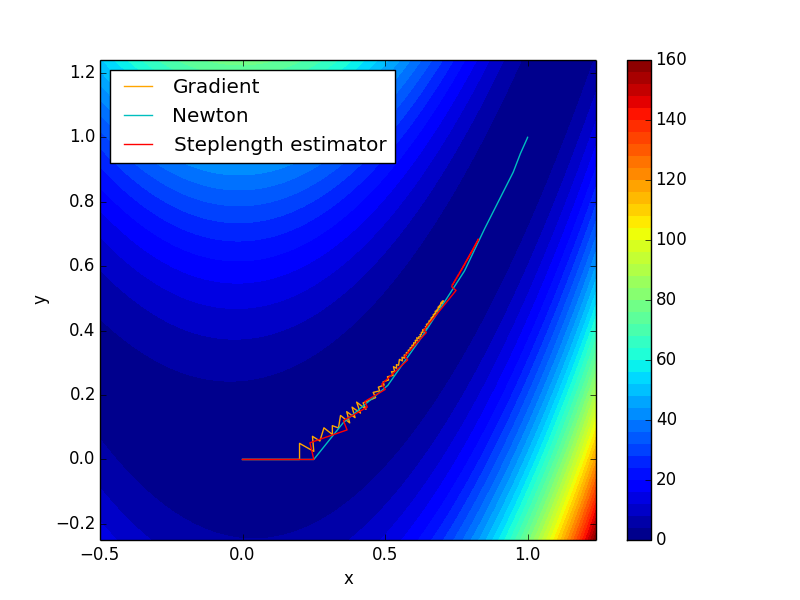
\includegraphics[height=6cm, width=8cm]{../src_rosen/Rosenbrock_iterations.png}
\caption{Comparison of iterations for minimizing the Rosenbrock function $(a=1.0, b=50.0)$ without noise. Comparisons are made between gradient descent, `Gradient', gradient descent with a line search estimator, `Steplength estimator', and full Newton scheme, `Newton'.}\label{Rosenbrock_iter1}
\end{figure}

\begin{figure}[!ht]
\centering
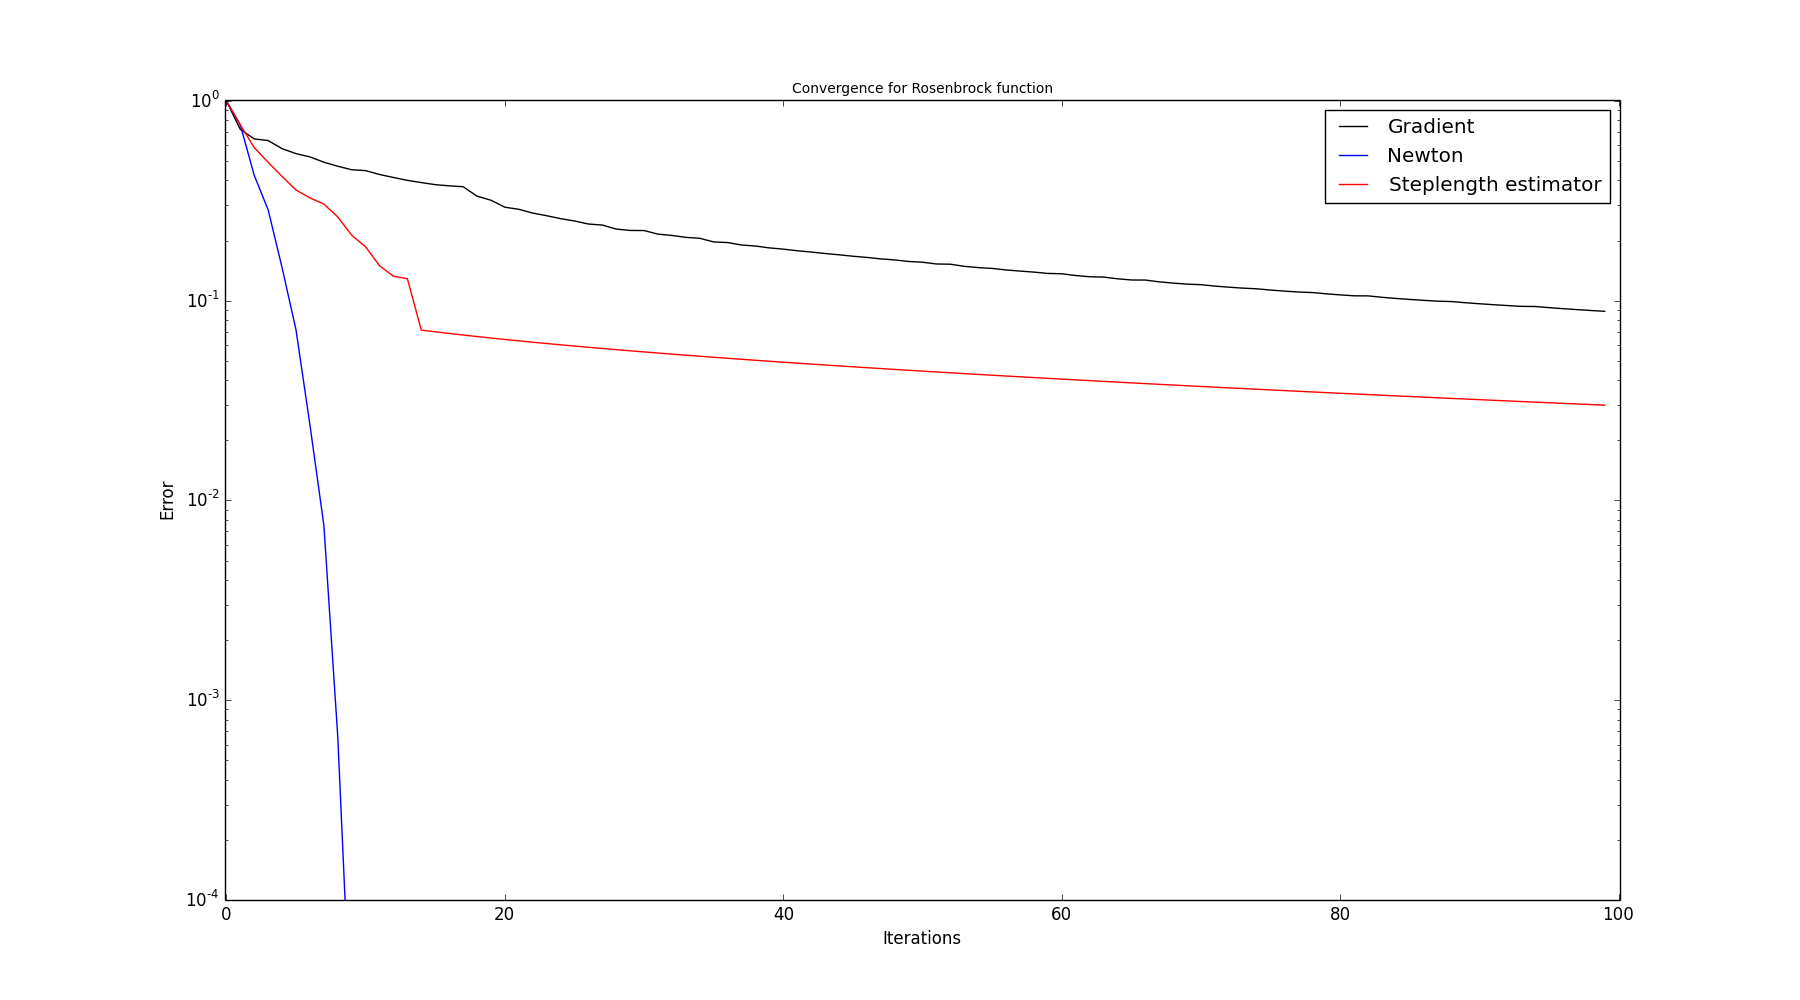
\includegraphics[height=6cm, width=8cm]{../src_rosen/Rosenbrock_convergence.png}
\caption{Convergence for minimization of the Rosenbrock function $(a=1.0, b=50.0)$ using, gradient descent, `Gradient', gradient descent with a line search estimator, `Steplength estimator', and full Newton scheme, `Newton'.}\label{Rosenbrock_conv1}
\end{figure}

\section{Method}
Succesfully training a neural network involves a number of components, an appropriate labelled dataset, the correct loss function and neural network architecture, a working solver for training the architecture and a well chosen evaluation metric.  For these reasons it is desirable to incrementally test each component. Testing will be carried out for two different different models, Logistic regression and softmax classification with a neural network doing this will validate aspects of the system. Logistic regression is a convex function but is trained by the same methods as non-convex neural networks. Therefore, testing with logistic regression validates that numerical optimization is implemented correctly. It also tests the viability of the stochastic sampling method. Neural networks are non-convex, and for a large dataset require batch sampling to train efficiently. Therefore, they represent a true test of optimization performance. 

All these components must be working for the system to be successful and errors in one aspect may obscure errors in another. For example, a large dataset which is well represented by its test set may hide a poor line-search implementation. Similarly, an inaccurate gradient may cause poor solver convergence, and stochastic sampling is likely to exacerbate any unresolved convergence issues. Furthermore, non-linear, non-convex objective functions are known to have saddle-points and local minima which can prevent convergence, or lead to convergence to the wrong minimum. Therefore, any bugs in the implementation risk being confused with a diagnosis of high-bias for a Neural network model.

\subsection{Data} 
When training the logistic regression classifier I used hand-made dataset consisting of 800 pairs of points in the $(x,y)$ plane each with a label, $0$ or $1$. Validation of the classifier (Tables \ref{table_stochlogreg_testerror} and \ref{table_sfixlogreg_testerror}) was carried out using the validation set which consists of 100 pairs of labelled points in the $(x,y)$ as illustrated in Figure \ref{valid_dataset}.

\begin{figure}[!ht]
\centering
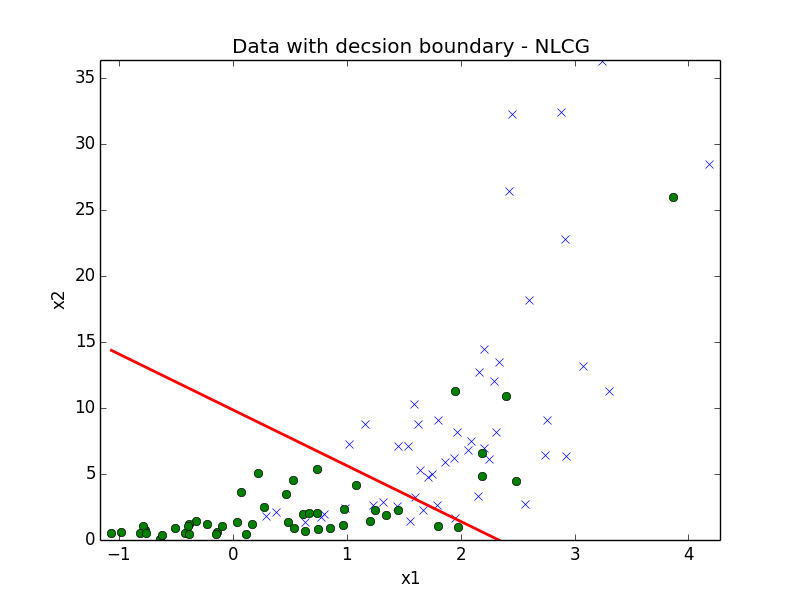
\includegraphics[height=6cm, width=8cm]{../src_logistic/logReg_pred_NLCG.png}
\caption{Validation dataset for Logistic regression with the decision boundary found by using an NLCG solver.}\label{valid_dataset}
\end{figure}

When experimenting with the neural network classifier I used Zalando's fashion MNIST dataset: \url{https://www.kaggle.com/zalando-research/fashionmnist}, \cite{FashionMNIST:data}. This dataset contains 60,000 training images and 10,000 testing images of clothing types, (labels: T-shirts, Trouser, Pullover, Dress, Coat, Sandal, Shirt, Sneaker, Bag, Ankle boot, with corresponding index numbered 0 - 9). Each image is 28 $\times$ 28 pixels in size, and is generally represented as a flat vector of 784 numbers. The dataset includes labels for each of the ten examples, a number indicating the actual clothing types (0 - 9) in that image. As the labels are not binary a multinomial loss function must be used.

\subsection{Models}   
This project will test convergence of various solvers for two loss functions, logistic loss and softmax (multinomial loss). In this section I define these loss-functions in terms of their weights (models).

\subsubsection*{Logistic regression}
Given data, $X \in \mathbb{R}^{(m,n)}$ consisting of $m$ examples each with $n$ features, and a set of $m$ binary classes for each example, $y\in \{0,1\}^{(m)}$, then we determine a model, $\theta \in \mathbb{R}^n$, which fits $X$ to $y$ by minimizing the logistic-loss, 
\begin{equation}
\mathcal{L}=-\frac{1}{m}\sum_{i}y^{(i)}\log{(\widehat{y}^{(i)})}+(1-y^{(i)})\log{(1-\widehat{y}^{(i)})}.\label{logistic_func}
\end{equation}
Where,
\begin{equation}
\widehat{y}=h_{\theta}(X)=\frac{1}{1+\exp(-X \theta)}.
\end{equation}
The gradient and Hessian of this function are given by,
\begin{align}
\nabla \mathcal{L}&=\frac{1}{m}X^{T}(h_{\theta}(X)-y),\\
\nabla^2 \mathcal{L}&=\frac{1}{m}X^{T}[h_{\theta}(X)(1-h_{\theta}(X))]X.
\end{align}
The Hessian is positive-semi definite and so $\mathcal{L}$ is convex with a well defined minimum. Hence, whilst this function is non-linear on its parameter $\theta$ an optimizer cannot become stuck in a local minima, though clearly some optimization methods will converge faster than others.
\subsubsection*{Neural Networks}
For good performance on Fashion MNIST logistic regression is unlikely to be sufficient. To increase model complexity, I will use a neural network consisting of $L$ layers with the weights of the layers being defined by a list of matrices, $W$ $(=[W_1,W_2,\ldots,W_L])$, and biases, $b$ $(=[b_1,b_2,\ldots,b_L])$. The forward propagation equation for the $l$-th layer takes the form,
\begin{align}
Z^{[l+1](i)}_j&=W^{[l+1]}_{j,k}X^{[l](i)}_k+b^{[l+1]}_j,  \label{propZ}\\
X^{[l+1](i)}_j&=\sigma^{[l+1]}(Z^{[l+1](i)}_j)\label{propX},
\end{align}
where $\sigma^{[l]}$ denotes the choice of activation function for the $l$-th layer. As mentioned, in Fashion MNIST each label is an integer representing a clothing type 0 - 9 and as such $y$ is a multinomial class (with $K=10$) rather than binary.  Therefore, at  the final layer, $L$ I will use the cross-entropy loss function,
\begin{equation}
\mathcal{L}=-\frac{1}{m}\sum_{i}\sum_{k=1}^{K} Y^{(i)}_k\log{(X^{[L](i)}_k)},\label{celossfunc}
\end{equation}
with
\begin{equation}
X^{[L]}=\sigma^{[L]}{(Z^{[L])})},
\end{equation}
where $\sigma^{[L]}$ is the softmax function, and $Y$ is the one-hot matrix representation of the multinomial classes. The final loss function is calculated using the `forward propagation' algorithm (algorithm \ref{alg:fwd}).

%If the $l$-th layer has $n_l$ features (with $n_0=n$) then,
%\begin{align}
%\textrm{shape}(X^{[l]})&=[n_l,m]=\textrm{shape}(Z^{[l]}),\\
%\textrm{shape}(W^{[l]})&=[n_l,n_{l-1}],\\
%\textrm{shape}(b^{[l]})&=[n_l,].
%\end{align}
%At the final layer we calculate the logistic-loss function,
%\begin{equation}
%\mathcal{L}=-\frac{1}{n}\sum_{i}y^{(i)}\log{(X^{[L](i)})}+(1-y^{(i)})\log{(1-X^{[L](i)})}.\label{lossfunc}
%\end{equation}
%
\begin{algorithm}
\caption{Forward propagation}\label{alg:fwd}
\begin{algorithmic}
\Procedure {forwardprop}{\textit{list(array)} $W=[W^1,W^2,\ldots, W^L]$,\textit{list(array)} $b=[b^1,b^2,\ldots, b^L]$,$\textit{array}(m,n)$ $X$, $\textit{array}(m)$ $y$}
	\State $X^{(0)} \gets X$
	\For {$l \leftarrow 1, L$}
		\State $Z^{(l)} \gets W^{(l)}X^{(l-1)}+b^{(l)}$
		\State $X^{(l)} \gets \sigma(Z^{(l)} )$
	\EndFor
	\State $\mathcal{L} \gets -\frac{1}{n} \textrm{sum}{\left[\log(X^{(L)})+(1-y)Z^{(L)}\right]}$
	\State \Return $\mathcal{L}$
\EndProcedure
\end{algorithmic}
\end{algorithm}

The gradient of the loss function with respect to the set of weights $W$, $\nabla \mathcal{L}$ $(=[\nabla \mathcal{L}^1_{W},\nabla \mathcal{L}^2_{W},\ldots,\nabla \mathcal{L}^L_{W}])$ are calculated by back-propagation. Starting from the final layer,
\begin{equation}
\left[\nabla \mathcal{L}^{[L]}
_{Z}\right]^{(i)}_k=\frac{1}{n}\left[X^{[L](i)}_k-y^{(i)}_k\right].\label{deriv_loss_final}
\end{equation}
The update equation are,
\begin{align}
[\nabla \mathcal{L}^{[l]}_{W}]_{j,k}&=X_{k}^{[l-1](i)}\left[\nabla \mathcal{L}^{[l]}_{Z}\right]^{(i)}_j,\label{gradW}\\
[\nabla \mathcal{L}^{[l]}_{b}]_j&=\sum_{i}\left[\nabla \mathcal{L}^{[l]}_{Z}\right]^{(i)}_j.\label{gradb}
\end{align}
and the backpropagation equation are,
\begin{align}
\left[ \nabla \mathcal{L}^{[l-1]}_{X}\right]^{(i)}_j&=\left(W^{T}\right)_{j,k}^{[l]}\left[\nabla \mathcal{L}^{[l]}_{Z}
\right]^{(i)}_k,\label{backprop_X}\\
\left[\nabla \mathcal{L}_{Z}^{[l-1]}\right]^{(i)}_j&= \sigma'{(Z_{j}^{[l-1](i)})}\left[\nabla \mathcal{L}_{X}^{[l-1]}\right]^{(i)}_j.\label{backprop_Z}\end{align}
Derivations of these equations are given in appendix \ref{backprop_derive}. These equation lead to the well-known `backward propagation' algorithm shown in algorithm \ref{alg:bwd}.
\begin{algorithm}
\caption{Backward propagation}\label{alg:bwd}
\begin{algorithmic}
\Procedure {backwardprop}{\textit{list(array)} $W=[W^1,W^2,\ldots, W^L]$,\textit{list(array)} $Z=[X^{[L]}, X^{[L-1]},\ldots,X^{[0]}$, $\textrm{array}(m)$ $y$}
	\State $\nabla \mathcal{L}^{[L]}_{Z} \gets \frac{1}{n}\left[X^{[L]}-y \right]$
	\For {$l \leftarrow L, 1$}
		\State $\nabla \mathcal{L}^{[l]}_{W} \gets  \nabla \mathcal{L}^{[l]}_{Z}X^{T[l-1]} $
		\State $\nabla \mathcal{L}^{[l]}_{b} \gets \textrm{sum}{(\nabla \mathcal{L}^{[l]}_{Z})}$
		\State $\nabla \mathcal{L}^{[l-1]}_{X} \gets W^{(l)T}\nabla \mathcal{L}^{[l]}_{Z}$
		\State $\nabla \mathcal{L}_{Z}^{[l-1]}\gets \sigma'{(Z^{[l-1]})} \nabla \mathcal{L}_{X}^{[l-1]}$
	\EndFor
	\State \Return $[\nabla \mathcal{L}^{[L]}_{W} , \nabla \mathcal{L}^{[L-1]}_{W}, \ldots,  \nabla \mathcal{L}^{[1]}_{W}]$, $[\nabla \mathcal{L}^{[L]}_{b} , \nabla \mathcal{L}^{[L-1]}_{b}, \ldots,  \nabla \mathcal{L}^{[1]}_{b}]$
\EndProcedure
\end{algorithmic}
\end{algorithm}
A Hessian can be calculated for each layer by taking second derivatives of equations \ref{deriv_loss_final}-\ref{backprop_Z}. The calculations are cumbersome and so the derivation of these equations, together with an algorithm for computing them, is presented in appendix \ref{Hess_prop}.

\subsection{Stochastic sampling strategy}\label{stoch_strategy}
In section \ref{results} we shall see that the stochastic sampling method has a significant influence on the success of higher-order methods. Given $m$ samples we define a batch $\mathcal{B}$ of size, $m_b$, to be a randomly chosen subset of $\{1,2,\ldots,m\}$ chosen without replacement. With this, $X^\mathcal{B}$, $y^\mathcal{B}$ denote a subsampling of the full data, $X$, and labels, $y$ with elements defined by the indices of the entries in  $\mathcal{B}$. The sampling is repeated a number, $R$, times to produce batches  $\mathcal{B}_1, \ldots, \mathcal{B}_R$. From this we define a stochastic objective function suitable for experimentation with a non-linear solver,
\begin{equation}
\mathcal{L}_{sub}(X,y)=\frac{1}{R}\sum_{r=1}^R \mathcal{L}(X^{\mathcal{B}_r}, y^{\mathcal{B}_r}).\label{stoch_resample}
\end{equation}
It would seem more correct to resample the batch $\mathcal{B}$ at each iteration. However, as mentioned by \cite{Martens:Deep} doing this breaks the assumptions of L-BFGS or NLCG and causes early termination of the solver. Therefore, each batch is fixed throughout training. It is also unnecessary to have repeated coverings of the input data, so in practice I use, $R=\lceil m/m_b \rceil$.

%\begin{algorithm}
%\caption{Backward propagation}\label{alg:bwd}
%\begin{algorithmic}
%\Procedure {backwardprop}{\textit{list(array)} $W=[W^1,W^2,\ldots, W^L]$,\textit{list(array)} $Z=[X^{[L]}, X^{[L-1]},\ldots,X^{[0]}$, $\textrm{array}(m)$ $y$}
%	\State $\nabla \mathcal{L}^{[L]}_{Z} \gets \frac{1}{n}\left[X^{[L]}-y \right]$
%	\For {$l \leftarrow L, 1$}
%		\State $\nabla \mathcal{L}^{[l]}_{W} \gets  \nabla \mathcal{L}^{[l]}_{Z}X^{T[l-1]} $
%		\State $\nabla \mathcal{L}^{[l]}_{b} \gets \textrm{sum}{(\nabla \mathcal{L}^{[l]}_{Z})}$
%		\State $\nabla \mathcal{L}^{[l-1]}_{X} \gets W^{(l)T}\nabla \mathcal{L}^{[l]}_{Z}$
%		\State $\nabla \mathcal{L}_{Z}^{[l-1]}\gets \sigma'{(Z^{[l-1]})} \nabla \mathcal{L}_{X}^{[l-1]}$
%	\EndFor
%	\State \Return $[\nabla \mathcal{L}^{[L]}_{W} , \nabla \mathcal{L}^{[L-1]}_{W}, \ldots,  \nabla \mathcal{L}^{[1]}_{W}]$, $[\nabla \mathcal{L}^{[L]}_{b} , \nabla \mathcal{L}^{[L-1]}_{b}, \ldots,  \nabla \mathcal{L}^{[1]}_{b}]$
%\EndProcedure
%\end{algorithmic}
%\end{algorithm}
\subsection{Evaluation metrics}
I will compare the performance of different solvers based on two metrics: the convergence of the solver during training and the bias-variance diagnostic. The former is the most important for distinguishing solvers as it dictates the rate of convergence. However, the latter is also important as a poorly chosen stochastic algorithm can converge well on a sample of the training set but have poor generalization error on the test set.  It is also good practice to perform a gradient test on any loss function used.  An inaccurate gradient may cause poor solver convergence, and stochastic sampling is likely to exacerbate any unresolved convergence issues. Furthermore, non-linear, non-convex objective functions are known to have saddle-points and local minima which can prevent convergence, or lead to convergence to the wrong minimum. Therefore, any bugs in the implementation risk being confused with a diagnosis of high-bias for a Neural network model.

\subsubsection*{Optimization convergence}\label{metric_conv_curve}
For each solver, the training error will be plotted against the number of iterations during training. This is the key metric for discriminating between solver choices. Better solvers will converge faster. Convergence is defined as the number of iterations, $k_{\epsilon}$, such that,
\begin{equation}
\| f(x_{k})-f(x_{k-1}) \| \le \epsilon.
\end{equation}

\subsubsection*{Bias-Variance Diagnostic}\label{bias_variance}
Dev (or test) accuracy can be defined by a sum over all samples within the dev (or test) set,
\begin{equation}
\textrm{accuracy}(x,y)=\frac{1}{m}\sum_{i=1}^{m}[y^{(i)}=\textrm{predict}(x^{(i)})].
\end{equation}
I will plot training error together with test accuracy for each choice of solver over a range of crucial hyper-parameters. Examples of these hyper-parameters are batch-size, $m_b$, regularization parameter, $\lambda$ and number of NN layers, $L$. For a purely convex function this test will not be informative since all solvers should converge to the same set of weights albeit at different rates. Thus, if all solvers achieve the same training error then the test error should also be the same for the same dataset. However, this is not necessarily the case when using stochastic sampling as a poorly chosen stochastic algorithm can converge well on a sample of the training set but have poor generalization error on the test set, see Table \ref{table_stochlogreg_testerror} for an example of this.

For a non-convex method the situation is more complicated. Here different solvers may converge to different minima and this impacts the bias-variance tradeoff. For example, if solver $A$ becomes trapped in a local minima whereas $B$ converges then the training error will be less for $A$. However, the solution for $B$ may actually overfit the data whereas $A$ does not. Here, $A$ will be exhibiting high-bias, lower-variance, whereas $B$ will show lower-bias, high-variance. In other words, $B$ is capable of simulating a larger range of models than $A$, therefore is increasing variance. For this reason, it is important to check bias-variance curves when comparing solvers on deep networks.
 
\subsubsection*{Gradient test}\label{grad_test}
Any objective function should be tested to ensure that for randomly chosen $m$ and $\Delta m$ and a suitably small $\epsilon$,
\begin{equation}
\frac{\mathcal{L}(m+\epsilon \Delta m)-\mathcal{L}(m-\epsilon \Delta m)}{2 \epsilon}=\Delta m^T \nabla \mathcal{L} + O(\epsilon^2). 
\end{equation}
 

%\subsection{Error Analysis}\label{err_analysis}
%Given,  data ($X \in \mathbb{R}^{(n,m)},$) and its labels ($y \in \mathbb{R}^m$) a working system must have at least three components,
%\begin{enumerate}
%\item An implementation of a loss function defined over a `model'. This includes,
%\begin{enumerate}
%\item A value of the loss function mapping a set of weights and biases $\mathcal{W}=[(W_1b_1),\ldots, (W_L,b_L)]$ to a (float) value,
%\begin{equation}
%\mathcal{L}: \mathcal{W} \to \mathbb{R}
%\end{equation}
%{\color{red}{[2] - largely implemented previously, though only in outline for deep nets}}, {\color{blue}{[5] - crucial}}.
%\label{objfn_item}
%\item Its gradient
%\begin{equation}
%\nabla \mathcal{L}: \mathcal{W} \to \mathcal{W},
%\end{equation}
%{\color{red}{[2] - largely implemented previously, though only in outline for deep nets}}, {\color{blue}{[5] -  crucial}}.
%
%\item {[Optional]} Its Hessian, or a means of approximating it,
% \begin{equation}
%\nabla^2 \mathcal{L}: \mathcal{W} \to \mathcal{W}\times \mathcal{W}.
%\end{equation}
%{\color{red}{[5] - the riskiest aspect, difficult to compute}}, {\color{blue}{[2] - would be interesting to test but not essential if using L-BFGS}}.\end{enumerate}
%\item A means for stochastically batch sampling the input data and interfacing this with the loss function. {\color{red}{[4] - risky, robust stochastic solvers is still a research question}}, {\color{blue}{[4] - this is necessary for training a large dataset}}.
%\item A classifier which includes,
%\begin{enumerate}
%\item A method for of fitting the data (calculating weights), using a solver (Gradient Descent, Newton's method with line search, NLCG or L-BFGS). {\color{red}{[3] - these functions exists in scipy}}, {\color{blue}{[4] - we dont need to compare all these options, but at least a couple}}.
%\item A method for generating predictions on unseen data. {\color{red}{[1] - already satisfied by \ref{objfn_item}}}, {\color{blue}{[1] - only important for bias-variance analysis}}.
%\end{enumerate}
%\end{enumerate}



\section{Results}\label{results}
\subsection{Logistic regression} 
In Figure \ref{Stoch_Logistic_regression_conv}, I compare the convergence rate between i. NLCG, ii. Newtons' method with line-search, iii. Newtons' method without line-search adaption, iv. L-BFGS during training on batches of the dataset using stochastic sampling. A batch size of 10 samples was chosen and the batches were reshuffled at each iteration. The sampling was repeated `Nbatches' times when calculating the objective function following the method of equation \ref{stoch_resample}. Note that due to reshuffling of the batches the NLCG and BFGS solvers terminated quickly. The corresponding test-error for this sampling method is shown in Table \ref{table_stochlogreg_testerror}
\begin{table}[h!]
\begin{center}
\begin{tabular}{ ccc} %\begin{tabular}{ |ccc|cc|c| } 
\hline
Solver & Train Loss & Test error  \\ 
\hline 
\hline
Newton (LS) & 0.4019 & 0.83\\ 
Newton (noLS) & 0.5613 & 0.81\\ 
L-BFGS & 0.6030 & \textbf{0.51}\\ 
NLCG & 0.5989 & \textbf{0.51}\\ 
\end{tabular}
\end{center}
\caption{Number of iterations and test error for stochastic logistic regression using a batch size of 10, with sampling repeated 50 times and using reshuffling at each iteration. Note that L-BFGS and NLCG have very poor performance on the test-set.}\label{table_stochlogreg_testerror}
\end{table}

In contrast to the reshuffling method, Figure \ref{StochFix_Logistic_regression_conv} shows the convergence rate for i. NLCG, ii. Newtons' method with line-search, iii. Newtons' method without line-search adaption, iv. L-BFGS during training.  A batch size of 10 samples was chosen and the batches were fixed throughout iteration. The sampling was not repeated, however 80 batches were used to cover the full training set.  The corresponding test-error for this sampling method is shown in Table \ref{table_sfixlogreg_testerror}

\begin{table}[h!]
\begin{center}
\begin{tabular}{ cccc} %\begin{tabular}{ |ccc|cc|c| } 
\hline
Solver & Niters & Train Loss & Test error  \\ 
\hline 
\hline
Newton (LS) & 8 & 0.4058 & 0.83\\ 
\textbf{Newton (noLS)} & \textbf{50} & \textbf{0.5617} & \textbf{0.81}\\ 
BFGS & 20 & 0.4058 & 0.83\\ 
NLCG & 31 & 0.4058 & 0.83\\ 
\end{tabular}
\end{center}
\caption{Number of iterations (`Niters')  and test error for logistic regression with a batch size of 10 using various solvers. Newton's method without line search shows higher bias due to early stopping.}\label{table_sfixlogreg_testerror}
\end{table}

\subsection{Fashion MNIST} 
In Figure \ref{NN_1layer} and \ref{NN_2layer} I compare the convergence rate between i.Gradient descent,  ii. NLCG and  iii. L-BFGS-B during training on batches of Fashion MNIST. The convergence on the dev set is shown and the train-dev accuracy is also plotted. In Figure \ref{NN_1layer}, one hidden layer was used, whereas in Figure \ref{NN_2layer} two hidden layers were used. A batch size of 1000 samples was chosen and the batches were fixed throughout each iteration. Whilst the train and dev curves are surprisingly close they are not exactly the same as is shown in Table \ref{table_fashion_mnist}. Comparisons of the runtime per iteration for each of these solvers is shown in Table \ref{rt_nn}.

\begin{table}[h!]
\begin{center}
\begin{tabular}{ ccc} %\begin{tabular}{ |ccc|cc|c| } 
\hline
Solver & Train Acc & Dev Acc  \\ 
\hline 
\hline
Gradient 1L & 0.7232 & 0.7195\\ 
NLCG 1L& 0.8363 & 0.8336\\ 
L-BFGS-B 1L& 0.8307 & 0.8293\\ 
Gradient 2L & 0.7029 & 0.7038\\ 
NLCG 2L& 0.7627 & 0.7650\\ 
L-BFGS-B 2L& 0.7782 & 0.7845\\ 
\end{tabular}
\end{center}
\caption{Train and Dev accuracy using 100 iterations on Fashion MNIST. $L$ stands for the number of hidden layers.}\label{table_fashion_mnist}
\end{table}

\begin{table}[h!]
\begin{center}
\begin{tabular}{ ccc} %\begin{tabular}{ |ccc|cc|c| } 
\hline
Solver & Runtime (s) & Runtime (s)  \\ 
& &per iteration \\
\hline 
\hline
Gradient 1L& 411.9 & 8.2\\ 
L-BFGS-B 1L& 569.3  & 11.3\\ 
NLCG 1L& 751.1 & 15.0 \\ 
Gradient 2L& 509.7 & 10.2 \\ 
L-BFGS-B 2L& 1010.1  & 20.2\\ 
NLCG 2L& 1215.2 & 24.3 \\ \end{tabular}
\end{center}
\caption{Runtime per iteration for 50 iterations with one (1L) or two (2L) hidden layers and regularization, $\lambda = 0.01$.}\label{rt_nn}
\end{table}

\section{Discussion}

 Figure \ref{Rosenbrock_conv1} shows that second order solvers have the ability to greatly outperform gradient descent. Figure \ref{StochFix_Logistic_regression_conv} shows that provided fixed batches are used, second order schemes with line-search outperform Newton methods without line searching. Indeed, the drastic improvement in convergence between using a line-search and fixed step size is striking. The explanation is that even with an accurate downhill step provided by the Newton method without any adjustment of the stepsize provided by a line search together with Wolfe conditions (see \cite{Nocedal:Wright}) the step length can be inappropriate leading to slow convergence. Note that because logistic regression does not contain any hidden layers, by batch sampling (with fixed batches) and then regathering all batches in the final objective function, as described by equation \ref{stoch_resample}, is equivalent to using all batches. This explains why convergence is regained once fixed batches were used.

For the case of training neural networks on Fashion MNIST the situation was less clear cut. It is noticeable that in early iterations the convergence was unstable (most likely the influence of batch sampling) and convergence took a while to `settle down'. However, there was a point when convergence for both L-BFGS and NLCG beat gradient descent and eventually settled down to convergence within 100 iterations whilst gradient descent had some way to go. Typically stochastic gradient descent schemes take upwards of $10^4$ iterations. Eventually, an accuracy of $0.83$ was achieved for both second-order solvers on both the test and dev set. It is also worrying that the statistics for the test and dev set accuracies and errors are so close. It is possible that this is a feature of the stochastic sampling method, but this matter needs further investigation as this could also be an error. The runtime of NLCG per iteration was almost twice that of gradient descent with L-BFGS-B coming in someway between. This higher cost per iteration might be considered less significant compared to the benefits gained by faster convergence.

\subsection{Future Work}
Three matters require further investigation. The most urgent of these is to explain the very close similarity between the train and dev accuracy and to determine if there is a bug here. 

Secondly, the results of the experiments on Fashion MNIST were somewhat inconclusive. The issue here is that the size of the Fashion MNIST dataset pushes us towards small batches, and so the influence of batch sampling outweighs improvements due purely to using improved solvers. Following on from the logistic regression case, I now think it would be beneficial to test neural networks on a smaller dataset where batch sampling is not immediately required. When this is done, it should be possible to progressively increase the deep of the network and in this way test for the onset of pathological convergence problems caused by saddle-points, and exploding-vanishing gradients. This would make a clearer test for the success of second-order schemes. 

Thirdly, my second order schemes do not make use of a preconditioner and in this sense are behind some other empirical studies in the literature such as those of \cite{Martens:Deep}, \cite{Xu:2ndNCML} and \cite{Asi:BetterStoch}. The equations derived in appendix \ref{Hess_prop} provide food for thought on this, and it is possible that simplifications of these equations may provide insights into effective preconditioning schemes for deep networks. Given the very preliminary results obtained in this work I humbly suggest this is worth pursuing. 

\newpage
\bibliographystyle{plain}
\bibliography{Milestone2_0}  




%\begin{figure}[!ht]
%\centering
%\includegraphics[height=6cm, width=8cm]{../src_rosen/Stochastic_Rosenbrock_iterations.png}
%\caption{Comparison of iterations for minimizing the Rosenbrock function $(a=1.0, b=50.0)$ with Gaussian noise added. Comparisons are made between gradient descent, `Gradient', gradient descent with a line search estimator, `Steplength estimator', and full Newton scheme, `Newton'.}\label{Rosenbrock_iter2}
%\end{figure}
%
%\begin{figure}[!ht]
%\centering
%\includegraphics[height=6cm, width=8cm]{../src_rosen/Stochastic_Rosenbrock_convergence_noise0pt01.png}
%\caption{Convergence for minimization of the Rosenbrock function $(a=1.0, b=50.0)$ with Gaussian noise added ($\sigma=0.01$). `Nbatches' refers to the number of times a batch is sampled, i.e. the number of calls to a noisy Rosenbrock function which were used to estimate an average value (or gradient). Comparisons are made between gradient descent, `Gradient', gradient descent with a line search estimator, `Steplength estimator', and full Newton scheme, `Hessian'.}\label{Rosenbrock_conv2}
%\end{figure}

%\begin{figure}[!ht]
%\centering
%\includegraphics[height=6cm, width=8cm]{../src_logistic/logreg_converge_test.png}
%\caption{Convergence of logistic regression during training for NLCG, Newtons' method with line-search, Newton (LS),  Newtons' method without line-search adaption,  Newton (noLS) and L-BFGS. Note that NLCG and L-BFGS curves lie on top of each other.}\label{Logistic_regression_conv}
%\end{figure}

\begin{figure}[!ht]
\centering
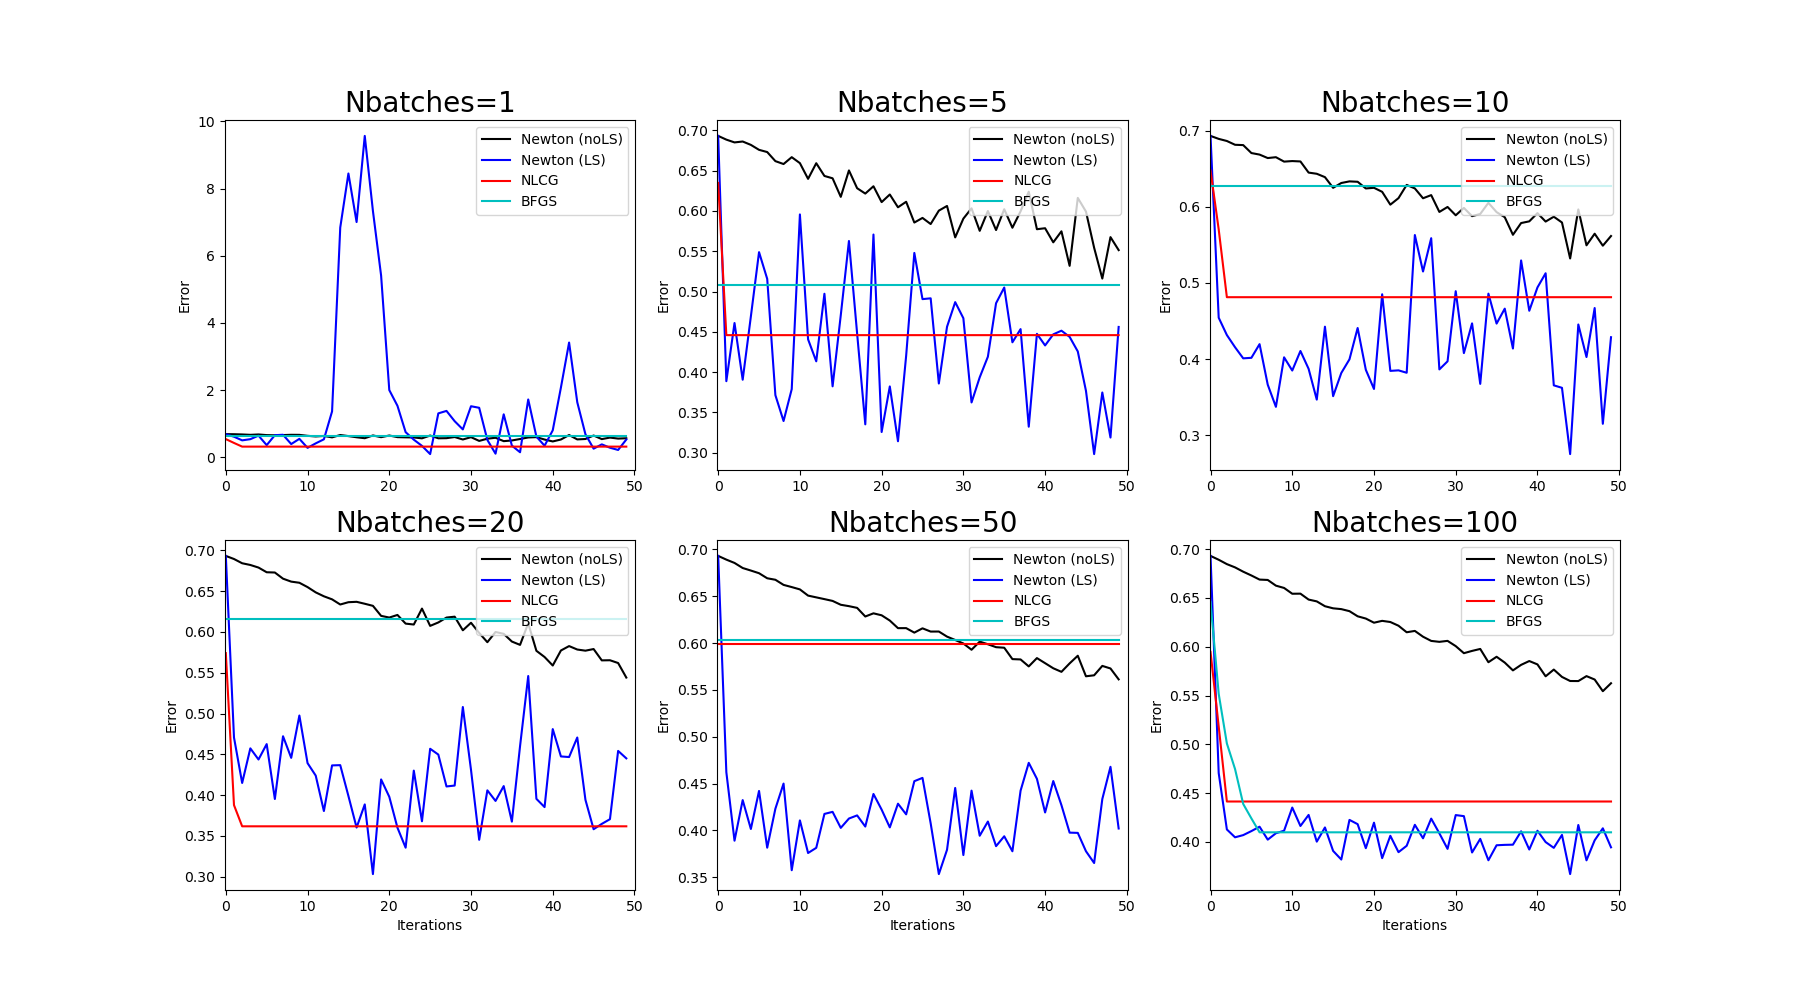
\includegraphics[height=6cm, width=8cm]{../src_logistic/stoch_logreg_converge_test_10.png}
\caption{Convergence of logistic regression during training with mini-batch sampling for NLCG, Newtons' method with line-search, Newton (LS),  Newtons' method without line-search adaption,  Newton (noLS) and L-BFGS. A batch size of 10 samples was chosen and `Nbatches' refers to the number of times the sampling is repeated (with reshuffling) when calculating the objective function defined in equation \ref{stoch_resample}.}\label{Stoch_Logistic_regression_conv}
\end{figure}

\begin{figure}[!ht]
\centering
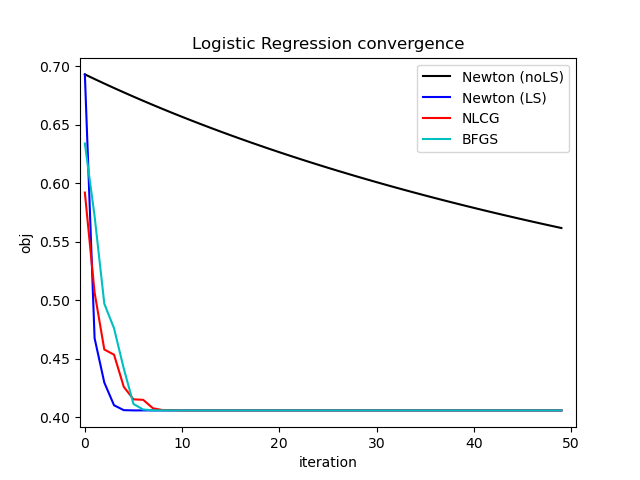
\includegraphics[height=6cm, width=8cm]{../src_logistic/stoch_logreg_converge_test_batch_size_10.png}
\caption{Convergence of logistic regression during training with mini-batch sampling of 10 samples for NLCG, Newtons' method with line-search, Newton (LS),  Newtons' method without line-search adaption,  Newton (noLS) and L-BFGS. Here the batches were fixed throughout training and $800/10=80$ batches were used.}\label{StochFix_Logistic_regression_conv}
\end{figure}

\begin{figure}[!ht]
\centering
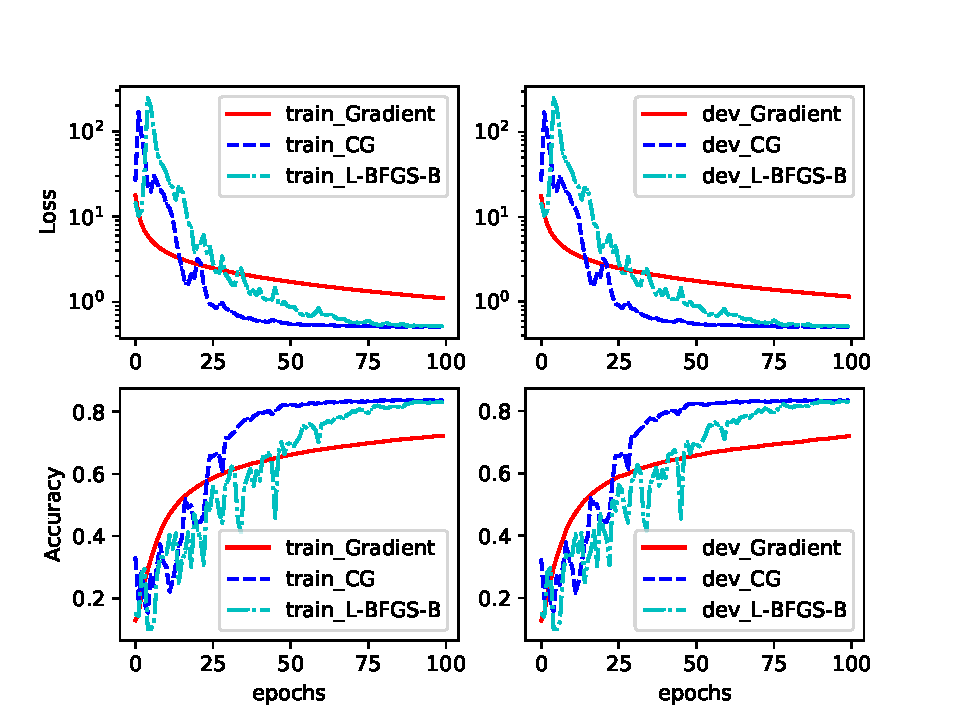
\includegraphics[height=6cm, width=8cm]{../src-mnist/compare_solvers_newtest_100_reg_0pt01_lr_0pt4.pdf}
\caption{Convergence of neural network during training on Fashion MNIST. Training was performed using one hidden layer, for 100 epochs with a batch size of 1000 samples and a regularization parameter, $\lambda=0.01$.}\label{NN_1layer}
\end{figure}

\begin{figure}[!ht]
\centering
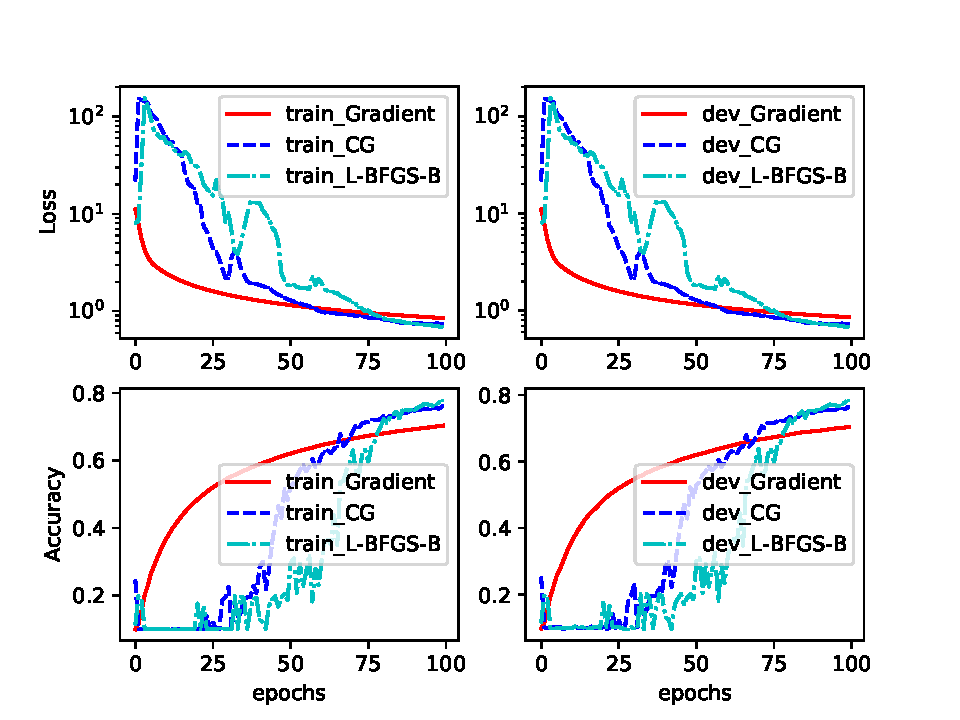
\includegraphics[height=6cm, width=8cm]{../src-mnist/compare_solvers_nL_2_nepoch_100_reg_0pt01_lr_0pt4.pdf}
\caption{Convergence of neural network during training on Fashion MNIST. Training was performed using two hidden layers, for 100 epochs with a batch size of 1000 samples and a regularization parameter, $\lambda=0.01$.}\label{NN_2layer}
\end{figure}

\newpage

%
%\begin{figure}[!ht]
%\centering
%\includegraphics[height=6cm, width=8cm]{../src/Rosenbrock_iterations_0pt005_momentum.png}
%\caption{Comparison of iterations for minimizing the Rosenbrock function $(a=1.0, b=50.0)$ with Gaussian noise added. Comparisons are made between gradient descent without momentum, `Gradient, no mom', and with momentum,  `Gradient, mom'.}\label{Rosenbrock_iter3}
%\end{figure}
%
%\begin{figure}[!ht]
%\centering
%\includegraphics[height=6cm, width=8cm]{../src/Rosenbrock_convergence_0pt005_momentum_vs_hess.png}
%\caption{Convergence for minimization of the Rosenbrock function $(a=1.0, b=50.0)$ with Gaussian noise added.  Comparisons are made between gradient descent with momentum, `Momentum' and full Newton scheme without momentum, `Hess, no mom'.}\label{Rosenbrock_conv3}
%\end{figure}



%\subsection{NN forward propagation step}
%Given data consisting of $m$ training examples with $n$ features, we denote the feature vector of the $i$-th training sample by  $X^{(i)}$. The NN will have $L$ layers with the weights of the layers being defined by a list of matrices, $W$ $(=[W_1,W_2,\ldots,W_L])$, and biases, $b$ $(=[b_1,b_2,\ldots,b_L])$. The forward propagation equation for the $l$-th layer takes the form,
%\begin{align}
%Z^{[l+1](i)}_j&=W^{[l+1]}_{j,k}X^{[l](i)}_k+b^{[l+1]}_j,  \label{propZ}\\
%X^{[l+1](i)}_j&=\sigma(Z^{[l+1](i)}_j)\label{propX},
%\end{align}
%where $\sigma$ denotes the sigmoid function, 
%\begin{equation}
%\sigma(z)=\frac{1}{1+e^{-z}}.
%\end{equation}
%Clearly, if the $l$-th layer has $n_l$ features (with $n_0=n$) then,
%\begin{align}
%\textrm{shape}(X^{[l]})&=[n_l,m]=\textrm{shape}(Z^{[l]}),\\
%\textrm{shape}(W^{[l]})&=[n_l,n_{l-1}],\\
%\textrm{shape}(b^{[l]})&=[n_l,].
%\end{align}
%At the final layer we calculate the logistic-loss function,
%\begin{equation}
%\mathcal{L}=-\frac{1}{n}\sum_{i}y^{(i)}\log{(X^{[L](i)})}+(1-y^{(i)})\log{(1-X^{[L](i)})}.\label{lossfunc}
%\end{equation}

%\begin{algorithm}
%\caption{Forward propagation}\label{alg:fwd}
%\begin{algorithmic}
%\Procedure {forwardprop}{\textit{list(array)} $W=[W^1,W^2,\ldots, W^L]$,\textit{list(array)} $b=[b^1,b^2,\ldots, b^L]$,$\textit{array}(m,n)$ $X$, $\textit{array}(m)$ $y$}
%	\State $X^{(0)} \gets X$
%	\For {$l \leftarrow 1, L$}
%		\State $Z^{(l)} \gets W^{(l)}X^{(l-1)}+b^{(l)}$
%		\State $X^{(l)} \gets \sigma(Z^{(l)} )$
%	\EndFor
%	\State $\mathcal{L} \gets -\frac{1}{n} \textrm{sum}{\left(y\log(X^{(L)})+(1-y)\log(1-X^{(L)})\right)}$
%	\State \Return $\mathcal{L}$
%\EndProcedure
%\end{algorithmic}
%\end{algorithm}

%\subsection{NN backward propagation step}
%We find the gradients of the loss function with respect to the set of weights $W$, $\nabla \mathcal{L}$ $(=[\nabla \mathcal{L}^1_{W},\nabla \mathcal{L}^2_{W},\ldots,\nabla \mathcal{L}^L_{W}])$. Starting from the final layer,
%\begin{equation}
%\left[\nabla \mathcal{L}^{[L]}
%_{Z}\right]^{(i)}=\frac{1}{n}\left[X^{[L](i)}-y^{(i)}\right].
%\end{equation}
%The update equation are,
%\begin{align}
%[\nabla \mathcal{L}^{[l]}_{W}]_{j,k}&=X_{k}^{[l-1](i)}\left[\nabla \mathcal{L}^{[l]}_{Z}\right]^{(i)}_j,\label{gradW}\\
%[\nabla \mathcal{L}^{[l]}_{b}]_j&=\sum_{i}\left[\nabla \mathcal{L}^{[l]}_{Z}\right]^{(i)}_j.\label{gradb}
%\end{align}
%and the backpropagation equation are,
%\begin{align}
%\left[ \nabla \mathcal{L}^{[l-1]}_{X}\right]^{(i)}_j&=\left(W^{T}\right)_{j,k}^{[l]}\left[\nabla \mathcal{L}^{[l]}_{Z}
%\right]^{(i)}_k,\label{backprop_X}\\
%\left[\nabla \mathcal{L}_{Z}^{[l-1]}\right]^{(i)}_j&= \sigma'{(Z_{j}^{[l-1](i)})}\left[\nabla \mathcal{L}_{X}^{[l-1]}\right]^{(i)}_j.\label{backprop_Z}\end{align}
%\begin{algorithm}
%\caption{Backward propagation}\label{alg:bwd}
%\begin{algorithmic}
%\Procedure {backwardprop}{\textit{list(array)} $W=[W^1,W^2,\ldots, W^L]$,\textit{list(array)} $Z=[X^{[L]}, X^{[L-1]},\ldots,X^{[0]}$, $\textrm{array}(m)$ $y$}
%	\State $\nabla \mathcal{L}^{[L]}_{Z} \gets \frac{1}{n}\left[X^{[L]}-y \right]$
%	\For {$l \leftarrow L, 1$}
%		\State $\nabla \mathcal{L}^{[l]}_{W} \gets  \nabla \mathcal{L}^{[l]}_{Z}X^{T[l-1]} $
%		\State $\nabla \mathcal{L}^{[l]}_{b} \gets \textrm{sum}{(\nabla \mathcal{L}^{[l]}_{Z})}$
%		\State $\nabla \mathcal{L}^{[l-1]}_{X} \gets W^{(l)T}\nabla \mathcal{L}^{[l]}_{Z}$
%		\State $\nabla \mathcal{L}_{Z}^{[l-1]}\gets \sigma'{(Z^{[l-1]})} \nabla \mathcal{L}_{X}^{[l-1]}$
%	\EndFor
%	\State \Return $[\nabla \mathcal{L}^{[L]}_{W} , \nabla \mathcal{L}^{[L-1]}_{W}, \ldots,  \nabla \mathcal{L}^{[1]}_{W}]$, $[\nabla \mathcal{L}^{[L]}_{b} , \nabla \mathcal{L}^{[L-1]}_{b}, \ldots,  \nabla \mathcal{L}^{[1]}_{b}]$
%\EndProcedure
%\end{algorithmic}
%\end{algorithm}
%\subsection{Hessian propagation}
%We continue the backward propagation equations to calculate the second derivatives. If we restrict attention to finding derivatives only between the hidden units in each layer rather than between layers, the latter being especially cumbersome and unnecessary for our purposes, then we are led to define the second order derivatives,
%\begin{align}
%(H_W^{[l]})_{jk,j'k'}&=\left(\frac{\partial^2 \mathcal{L}}{\partial W^{[l]}_{j,k} \partial W^{[l]}_{j',k'}}\right)\label{H_W}\\
%(H_b^{[l]})_{j,j'}&=\left(\frac{\partial^2 \mathcal{L}}{\partial b_{j} \partial b_{j'}}\right)^{[l]}\\
%(H_{Wb}^{[l]})_{jk,j'}&=\left(\frac{\partial^2 \mathcal{L}}{\partial W^{[l]}_{j,k} \partial b^{[l]}_{j'}}\right)\\
%(H_Z^{[l]})^{(i)}_{p,q}&=\left(\frac{\partial^2 \mathcal{L}}{\partial Z_{p}^{[l](i)} \partial Z_{q}^{[l](i)}}\right)\\
%(H_X^{[l]})^{(i)}_{p,q}&=\left(\frac{\partial^2 \mathcal{L}}{\partial X_{p}^{[l](i)} \partial X_{q}^{[l](i)}}\right)\label{H_X}
%\end{align}
%Under these definitions a Hessian for each layer can be calculated from\footnote{See equations \ref{H_W_final}, \ref{H_Wb_final}, \ref{H_b_final} in appendix  \ref{Hess_prop}. },
%\begin{align}
%H_W^{[l]}&=(I_{n_l,n_l} \otimes X^{[l-1]})\Diag{(H_Z^{[l](0)},H_Z^{[l](1)},\ldots,H_Z^{[l](m)})}(I_{n_l,n_l} \otimes X^{[l-1]})^T,\label{H_W_calc}\\
%H_{Wb}^{[l]}&=(I_{n_l,n_l} \otimes X^{[l-1]}) [H_Z^{[l](0)},H_Z^{[l](1)},\ldots,H_Z^{[l](m)}]^T\label{H_Wb_calc}\\
%H_{b}^{[l]}&=\sum_i H_Z^{[l](i)}.\label{H_Wb_calc}
%\end{align}
%As in the case of back-propagation the $H_Z^{[l]}$ can be back-propagated through the layers by the rules\footnote{See equation \ref{H_X_final} and \ref{H_Z_final}},
%\begin{align}
%H_X^{[l-1]}&=W^{[l]T} H_Z^{[l]}W^{[l]}.\label{H_X_backprop}\\
%H_Z^{[l-1]}&=\sigma'{(Z^{[l-1]})}\circ H_X^{[l-1]} \circ \sigma'{(Z^{[l-1]})}\color{red}{+\sigma''{(Z^{[l-1]})}\circ \Diag{\left(\nabla \mathcal{L}^{[l]}_{X}\right)}},\label{H_Z_backprop},
%\end{align}
%starting from,
%\begin{equation}
%H_Z^{[L]}=\frac{1}{n}\sigma'{(Z^{[L]})}\label{H_Z_initial}.
%\end{equation}
%A derivation of these statements is given in appendix \ref{Hess_prop}. 
\hrule  
\appendix
\section{Derivation of backward propagation equations}\label{backprop_derive}
Starting from the definition of the cross-entropy loss function \ref{celossfunc}, 
\begin{equation}
\left(\frac{\partial \mathcal{L}}{\partial X}\right)^{[L](i)}_k=-\frac{1}{m}\frac{y^{(i)}_k}{X^{[L](i)}_k},
\end{equation}
and so, by the chain-rule the derivatives with respect to $Z$ are,
\begin{equation}
\left(\frac{\partial \mathcal{L}}{\partial Z}\right)^{[L](i)}_k=\left(\frac{\partial \mathcal{L}}{\partial X}\right)^{[L](i)}_r \left(\frac{\partial X^{[L](i)}_r}{\partial Z^{[L](i)}_k}\right),
\end{equation}
with,
\begin{equation}
\left(\frac{\partial X^{[L](i)}_r}{\partial Z^{[L](i)}_k}\right)=X_{r}^{[L]i}(\delta_{k,r} - X_{k}^{[L]i}).
\end{equation}
Therefore,
\begin{equation}
\left(\frac{\partial \mathcal{L}}{\partial Z}\right)^{[L](i)}_k=\frac{1}{m}\left[X^{[L](i)}_k-y^{(i)}_k\right].
\end{equation}
Now using the chain-rule for the weights derivatives,
\begin{align}
\left(\frac{\partial \mathcal{L}}{\partial W_{j,k}}\right)^{[l]}&=\sum_{i,p}\left(\frac{\partial \mathcal{L}}{\partial Z_{p}}\right)^{[l](i)}\left(\frac{\partial Z_{p}^{[l](i)}}{\partial W_{j,k}^{[l]}}\right),\label{dL_dW}\\
\left(\frac{\partial \mathcal{L}}{\partial b_{j}}\right)^{[l]}&=\sum_{i,p}\left(\frac{\partial \mathcal{L}}{\partial Z_{p}}\right)^{[l](i)}\left(\frac{\partial Z_{p}^{[l](i)}}{\partial b_{j}^{[l]}}\right).\label{dL_db}
\end{align}
By equation \ref{propZ},
\begin{align}
\frac{\partial Z_{p}^{[l](i)}}{\partial W_{j,k}^{[l]}}&=\delta_{p,j}X_{k}^{[l-1](i)},\label{dZ_dW}\\
\frac{\partial Z_{p}^{[l](i)}}{\partial b_{j}^{[l]}}&=\delta_{p,j},\label{dZ_db}\\
\left(\frac{\partial Z_{p}^{[l]}}{\partial X_{k}^{[l-1]}}\right)^{(i)}&=W_{p,k}^{[l]}.\label{dZ_dX}
\end{align}
Substituting \ref{dZ_dW} into \ref{dL_dW}, and \ref{dZ_db} into \ref{dL_db} leads to,
\begin{align}
\left(\frac{\partial \mathcal{L}}{\partial W_{j,k}}\right)^{[l]}&=\sum_{i}\left(\frac{\partial \mathcal{L}}{\partial Z_{j}}\right)^{[l](i)}X_{k}^{[l-1](i)}\\
&=X_{k}^{[l-1],T}\left(\frac{\partial \mathcal{L}}{\partial Z_{j}}\right)^{[l]},\label{wts_update}\\
\left(\frac{\partial \mathcal{L}}{\partial b_{j}}\right)^{[l]}&=\sum_{i}\left(\frac{\partial \mathcal{L}}{\partial Z_{j}}\right)^{[l](i)}\label{bias_update}.
\end{align}
Whilst from equation \ref{dZ_dX},
\begin{align}
\left(\frac{\partial \mathcal{L}}{\partial X_{k}}\right)^{[l-1](i)}&=\sum_{p}\left(\frac{\partial \mathcal{L}}{\partial Z_{p}}\right)^{[l](i)}\left(\frac{\partial Z_{p}^{[l](i)}}{\partial X_{k}^{[l-1](i)}}\right),\\
&=\sum_{p} W_{p,k}^{[l]}\left(\frac{\partial \mathcal{L}}{\partial Z_{p}}\right)^{[l](i)},\\
&=\left(W^{T}\right)_{k,p}^{[l]}\left(\frac{\partial \mathcal{L}}{\partial Z_{p}}
\right)^{[l](i)}\label{backprop_dL_dX}.
\end{align}
Finally, from equation \ref{propX},
\begin{align}
\left(\frac{\partial \mathcal{L}}{\partial Z_{k}}\right)^{[l-1](i)}&=\sum_{p}\left(\frac{\partial \mathcal{L}}{\partial X_{p}}\right)^{[l-1](i)}\left(\frac{\partial X_{p}^{[l-1](i)}}{\partial Z_{k}^{[l-1](i)}}\right),\\
&= \sigma'{(Z_{k}^{[l-1](i)})}\left(\frac{\partial \mathcal{L}}{\partial X_{k}}\right)^{[l-1](i)}\label{backprop_dL_dZ}
\end{align}
Equations \ref{backprop_dL_dX} and \ref{backprop_dL_dZ} are the back-propagation equations used in equations \ref{backprop_X} and \ref{backprop_Z} respectively within the main text. Equations \ref{wts_update} and \ref{bias_update} define the updates for the weights and biases as used in equations \ref{gradW} and \ref{gradb}.These equations lead to the back-propagation algorithm shown in algorithm \ref{alg:bwd} 

\onecolumn
\section{Second-order derivatives}\label{Hess_prop}
We continue the backward propagation equations to calculate the second derivatives. If we restrict attention to finding derivatives only between the hidden units in each layer rather than between layers, then we are led to define the second order derivatives,
\begin{align}
(H_W^{[l]})_{jk,j'k'}&=\left(\frac{\partial^2 \mathcal{L}}{\partial W^{[l]}_{j,k} \partial W^{[l]}_{j',k'}}\right)\label{H_W}\\
(H_b^{[l]})_{j,j'}&=\left(\frac{\partial^2 \mathcal{L}}{\partial b_{j} \partial b_{j'}}\right)^{[l]}\\
(H_{Wb}^{[l]})_{jk,j'}&=\left(\frac{\partial^2 \mathcal{L}}{\partial W^{[l]}_{j,k} \partial b^{[l]}_{j'}}\right)\\
(H_Z^{[l]})^{(i)}_{p,q}&=\left(\frac{\partial^2 \mathcal{L}}{\partial Z_{p}^{[l](i)} \partial Z_{q}^{[l](i)}}\right)\\
(H_X^{[l]})^{(i)}_{p,q}&=\left(\frac{\partial^2 \mathcal{L}}{\partial X_{p}^{[l](i)} \partial X_{q}^{[l](i)}}\right)\label{H_X}
\end{align}
Under these definitions a Hessian for each layer can be calculated from the backpropagation equations by calculating second-order derivatives,
\begin{align}
\left(\frac{\partial^2 \mathcal{L}}{\partial W_{j,k} \partial W_{j',k'}}\right)^{[l]}&=\left(\frac{\partial^2 \mathcal{L}}{\partial Z_{j}\partial Z_{j'}}\right)^{[l](i)}X_{k}^{[l-1](i)}X_{k'}^{[l-1](i)},\\
&=X_{k}^{[l-1],T}\left(\frac{\partial^2 \mathcal{L}}{\partial Z_{j}\partial Z_{j'}}\right)^{[l]}X_{k'}^{[l-1]},\label{d2L_dW2}\\
\left(\frac{\partial^2 \mathcal{L}}{\partial b_{j}\partial b_{j'}}\right)^{[l]}&=\sum_{i}\left(\frac{\partial^2 \mathcal{L}}{\partial Z_{j} \partial Z_{j'} }\right)^{[l](i)},\label{d2L_db2}\\
\left(\frac{\partial^2 \mathcal{L}}{\partial W_{j,k} \partial b_{j'}}\right)^{[l]}&=\sum_{i}\left(\frac{\partial^2 \mathcal{L}}{\partial Z_{j}\partial Z_{j'}}\right)^{[l](i)}X_{k}^{[l-1](i)},\\
&=X_{k}^{[l-1],T}\left(\frac{\partial^2 \mathcal{L}}{\partial Z_{j}\partial Z_{j'}}\right)^{[l]}\label{d2L_dWdb},
\end{align}
Equations \ref{d2L_dW2}, \ref{d2L_db2} and \ref{d2L_dWdb} define the Hessian matrix of the weights and biases. Whilst, for the hideen layers $X^{[l-1]}$,
\begin{align}
\left(\frac{\partial^2 \mathcal{L}}{\partial X_{k}\partial X_{k'}}\right)^{[l-1](i)}
&=\sum_{p,q} W_{p,k}^{[l]}\left(\frac{\partial^2 \mathcal{L}}{\partial Z_{p} Z_{q}}\right)^{[l](i)}\left(\frac{\partial Z_{q}^{[l](i)}}{\partial X_{k'}^{[l-1](i)}}\right),\\
&=\sum_{p,q} W_{p,k}^{[l]}\left(\frac{\partial^2 \mathcal{L}}{\partial Z_{p} Z_{q}}\right)^{[l](i)}W_{q,k'}^{[l]},\\
&=\left(W^{T}\right)_{k,p}^{[l]}\left(\frac{\partial^2 \mathcal{L}}{\partial Z_{p} \partial Z_{q}}\right)^{[l](i)} W_{q,k'}^{[l]}\label{d2L_dX2}.
\end{align}
Hence, for $Z^{[l-1]}$,
\begin{align}
\left(\frac{\partial^2 \mathcal{L}}{\partial Z_{k} \partial Z_{k'}}\right)^{[l-1](i)}=& \sigma'{(Z_{k}^{[l-1](i)})}\left(\frac{\partial^2 \mathcal{L}}{\partial X_{k}\partial X_{k'}}\right)^{[l-1](i)} \left(\frac{\partial X_{k'}^{[l-1](i)}}{\partial Z_{k'}^{[l-1](i)}}\right)\\
&+\sigma''{(Z_{k}^{[l-1](i)})}\delta_{k,k'}\left(\frac{\partial \mathcal{L}}{\partial X_{k}}\right)^{[l-1](i)}\\
=&\sigma'{(Z_{k}^{[l-1](i)})}\left(\frac{\partial^2 \mathcal{L}}{\partial X_{k}\partial X_{k'}}\right)^{[l-1](i)} \sigma'{(Z_{k'}^{[l-1](i)})}\\
&+\sigma''{(Z_{k}^{[l-1](i)})}\delta_{k,k'}\left(\frac{\partial \mathcal{L}}{\partial X_{k}}\right)^{[l-1](i)}\label{d2L_dZ2}
\end{align}
equations \ref{d2L_dX2} and \ref{d2L_dZ2} define the propagation equations,
\begin{align}
(H_X^{[l-1](i)})_{k,k'}&=\left(W^{T}\right)_{k,p}^{[l]} (H_Z^{[l](i)})_{p,q}W_{q,k'}^{[l]}.\label{backprop_HX}\\
(H_Z^{[l-1](i)})_{k,k'}&=\sigma'{(Z_{k}^{[l-1](i)})}(H_X^{[l-1](i)})_{k,k'} \sigma'{(Z_{k'}^{[l-1](i)})}+\sigma''{(Z_{k}^{[l-1](i)})}\delta_{k,k'}\left(\frac{\partial \mathcal{L}}{\partial X_{k}}\right)^{[l-1](i)}\label{backprop_HZ}.
%(H_Z^{[l-1](i)})_{k,k'}&=\sigma'{(Z_{k}^{[l-1](i)})}\left(W^{T}\right)_{k,p}^{[l]} (H_Z^{[l](i)})_{p,q}W_{q,k'}^{[l]}\sigma'{(Z_{k'}^{[l-1](i)})}+\sigma''{(Z_{k}^{[l-1](i)})}\delta_{k,k'}\left(W^{T}\right)_{k,p}^{[l]}\left[\nabla \mathcal{L}^{[l]}_{Z}\right]^{(i)}_p.
\end{align}
Leading to the weights updates,
\begin{align}
(H_W^{[l]})_{jk,j'k'}&=\sum_{i}X_{k}^{[l-1](i)}(H_Z^{[l]})^{(i)}_{j,j'}X_{k'}^{[l-1](i)},\\
(H_{Wb}^{[l]})_{jk,j'}&=\sum_{i}X_{k}^{[l-1](i)}(H_Z^{[l]})^{(i)}_{j,j'},\\
(H_b^{[l]})_{j,j'}&=\sum_{i}(H_Z^{[l]})^{(i)}_{j,j'}.\label{H_b_final}
\end{align}
To simplify these expressions I will define\footnote{$A \otimes B$ denotes the tensor product,
\begin{equation}
A \otimes B=\left[\begin{array}{cccc}
A b_{11} & A b_{12} & \ldots  &A b_{1n}\\
A b_{21} & A b_{22} & \ldots &A b_{2n}\\
\vdots & \vdots & \ddots &\vdots\\
A b_{m1} & A b_{m2} & \ldots &A b_{mn}\\
\end{array}
\right].
\end{equation}},
\begin{align}
(H_W^{[l]})_{jk,j'k'}&=\sum_{pi,p'i'}\delta_{j,p}X_{k}^{[l-1](i)}((H_Z)^{[l](i)}_{p,p'}\delta^{i,i'})X_{k'}^{[l-1](i')}\delta_{j',p'},\\
&=\sum_{pi,p'i'}(I_{n_l,n_l} \otimes X^{[l-1]})_{jk,pi}((H_Z)^{[l](i)}_{p,p'}\delta^{i,i'})(I_{n_l,n_l} \otimes X^{[l-1]})_{j'k',p'i'},\\
&=\sum_{pi,p'i'}(I_{n_l,n_l} \otimes X^{[l-1]})_{jk,pi}((H_Z)^{[l](i)}_{p,p'}\delta^{i,i'})(I_{n_l,n_l} \otimes X^{[l-1]})^T_{p'i',j'k'}\\
(H_{Wb}^{[l]})_{jk,j'}&=\sum_{i}X_{k}^{[l-1](i)}(H_Z^{[l]})^{(i)}_{j,j'}.\\
&=\sum_{i,p}\delta_{j,p} X_{k}^{[l-1](i)}(H_Z^{[l]})^{(i)}_{p,j'}.\\
&=\sum_{i,p}(I_{n_l,n_l} \otimes X^{[l-1]})_{jk,pi}(H_Z^{[l]})^{(i)}_{p,j'}.
\end{align} 
From these equations we can calculate a Hessian for each layer from,
\begin{align}
H_W^{[l]}&=(I_{n_l,n_l} \otimes X^{[l-1]})\Diag{(H_Z^{[l](0)},H_Z^{[l](1)},\ldots,H_Z^{[l](m)})}(I_{n_l,n_l} \otimes X^{[l-1]})^T,\label{H_W_calc}\\
H_{Wb}^{[l]}&=(I_{n_l,n_l} \otimes X^{[l-1]}) [H_Z^{[l](0)},H_Z^{[l](1)},\ldots,H_Z^{[l](m)}]^T\label{H_Wb_calc}\\
H_{b}^{[l]}&=\sum_i H_Z^{[l](i)}.\label{H_b_calc}
\end{align}
As in the case of back-propagation the $H_Z^{[l]}$ can be back-propagated through the layers following the update rules,
\begin{align}
H_X^{[l-1]}&=W^{[l]T} H_Z^{[l]}W^{[l]}.\label{H_X_backprop}\\
H_Z^{[l-1]}&=\sigma'{(Z^{[l-1]})}\circ H_X^{[l-1]} \circ \sigma'{(Z^{[l-1]})}\color{red}{+\sigma''{(Z^{[l-1]})}\circ \Diag{\left(\nabla \mathcal{L}^{[l]}_{X}\right)}},\label{H_Z_backprop},
\end{align}
starting from,
\begin{equation}
H_{Z,p,q}^{[L](i)}=\frac{1}{m} X^{[L](i)}_p\left(\delta_{p,q}-X^{[L](i)}_q \right)\label{H_Z_initial}.
\end{equation}
From these equations an algorithm can be devised for back-propagating the Hessian from layer $L$ to $1$, this is outlined in Algorithm \ref{alg:backhess}
%and the Hessian terms are,
%\begin{align}
%(H_W^{[l]})&=(X^{[l-1]}\otimes I)\cdot \Diag{(I \otimes H_Z^{[l]})}\cdot (X^{[l-1]}\otimes I)^{T},\\
%(H_{Wb}^{[l]})&=(I \otimes H_Z^{[l]})\cdot (X^{[l-1]}\otimes I)^{T},\\
%(H_b^{[l]})&=\sum_{i}(H_Z^{[l]})^{(i)}.
%\end{align}
\begin{algorithm}
\caption{Backward propagation with Hessian}\label{alg:backhess}
\begin{algorithmic}
\Procedure {backwardhessprop}{\textit{list(array)} $W=[W^1,W^2,\ldots, W^L]$,\textit{list(array)} $Z=[X^{[L]}, X^{[L-1]},\ldots,X^{[0]}$, $\textrm{array}(m)$ $y$}
	\State $\nabla \mathcal{L}^{[L]}_{Z} \gets \frac{1}{n}\left[X^{[L]}-y \right]$
	\State $H^{[L]}_{Z} \gets \frac{1}{n}(Z^{L})(1-Z^{L})$	
	\For {$l \leftarrow L, 1$}
		\State $\nabla \mathcal{L}^{[l]}_{W} \gets  \nabla \mathcal{L}^{[l]}_{Z}X^{T[l-1]} $
		\State $\nabla \mathcal{L}^{[l]}_{b} \gets \textrm{sum}{(\nabla \mathcal{L}^{[l]}_{Z})}$
		\State $[H^{[l]}_W,H^{[l]}_{Wb},H^{[l]}_b] \gets \textrm{Hess}(H^{[l]}_Z, X^{[l-1]})$
		\State \Comment $\textrm{shape}(H^{[l]}_W)=[n_{l}n_{l-1},n_{l}n_{l-1}]$
		\State \Comment $\textrm{shape}(H^{[l]}_{Wb})=[n_{l}n_{l-1},n_{l}]$
		\State \Comment $\textrm{shape}(H^{[l]}_{b})=[n_{l},n_{l}]$			
		\State $H^{[l]} \gets [[H^{[l]}_W,H^{[l]}_{Wb}],[H^{[l]T}_{Wb},H^{[l]}_b]]$	
		\State $\nabla \mathcal{L}^{[l-1]}_{X} \gets W^{(l)T}\nabla \mathcal{L}^{[l]}_{Z}$
		\State $H^{[l-1]}_{X} \gets W^{(l)T} H_Z^{[l]}W^{[l]}$			
		\State \Comment As shapes: $[n_{l-1},m,n_{l-1}] \gets [n_{l-1},n_l] [n_{l},m,n_{l}] [n_l, n_{l-1}]$	
		\State $\nabla \mathcal{L}_{Z}^{[l-1]}\gets \sigma'{(Z^{[l-1]})} \nabla \mathcal{L}_{X}^{[l-1]}$
		\State $H^{[l-1]}_{Z} \gets \sigma'{(Z^{[l-1]})} H_X^{[l-1]}  \sigma'{(Z^{[l-1]})}+\sigma''{(Z^{[l-1]})} \Diag{\left(\nabla \mathcal{L}^{[l]}_{X}\right)}$
		\State \Comment As shapes: $[n_{l-1},m,n_{l-1}] \gets [n_{l-1},m,n_{l-1}] + [n_{l-1},m,n_{l-1}] $	
	\EndFor
	\State \Return $[[\nabla \mathcal{L}^{[L]}_{W} ,\mathcal{L}^{[L]}_{b} ],[ \nabla \mathcal{L}^{[L-1]}_{W},  \nabla \mathcal{L}^{[L-1]}_{b}]\ldots, [ \nabla \mathcal{L}^{[1]}_{W}, \nabla \mathcal{L}^{[1]}_{b}]]$, $[H^{[L]} ,H^{[L-1]}, \ldots, H^{[1]}]$
\EndProcedure
\Statex
\Procedure {Hess}{$H^{[l]}_Z$, $X^{[l-1]}$}
	\State $[n_{l},m,n_{l}] \gets \textrm{shape}(H^{[l]}_Z)$, $[n_{l-1},m] \gets \textrm{shape}(X^{[l-1]})$
	\State $Y \gets np.kron(I(n_{l},n_{l}),X^{[l-1]})$
	\State $D \gets np.zeros(n_l \times m, n_l \times m)$
	\State $E \gets np.zeros(n_l \times m, n_l)$	
	\For {$i \leftarrow 0, m$}
		\State $D[i n_l:(i+1) n_l, i n_l:(i+1) n_l] \gets H^{[l]}_Z[:,i,:]$
		\State $E[i n_l:(i+1) n_l, n_l] \gets H^{[l]}_Z[:,i,:]$	
	\EndFor
	\State $H^{[l]}_W \gets Y \times D \times Y^T$
	\State $H^{[l]}_{Wb} \gets Y \times E$
	\State $H^{[l]}_{b} \gets \textrm{sum}(H^{[l]}_Z[:,i,:],i)$
	\State \Return $[H^{[l]}_W, H^{[l]}_{Wb}, H^{[l]}_{b} ]$	
\EndProcedure
\end{algorithmic}
\end{algorithm}
\twocolumn
\section{A remark on convexity}\label{app_convex}
By inspection of equations \ref{H_W_calc}-\ref{H_Z_backprop} we note that with the exception of the term in red in equation \ref{H_Z_backprop} that every term is of the form\footnote{Care must be taken with equation \ref{H_Z_initial}. However, it is positive semi-definite because,
\begin{align}
y^T H_{Z}^{[L](i)}y&=\frac{1}{m} \sum_p  X^{[L](i)}_p y_p^2 -(\sum_q X^{[L](i)}_p y_p)^2,\\
&=\frac{1}{m} \sum_p X^{[L](i)}_p(y_p-\sum_q X^{[L](i)}_q y_q)^2
\end{align}
The last expression is $\ge 0$ since $X^{[L](i)}_p \ge 0$.}, $x^{T}Hx$. Furthermore, the procedure is iterative starting from equation \ref{H_Z_initial} and since 
\begin{equation}
\sigma'(z) >0 \hspace{0.2cm} \forall z \in \mathbf{R},
\end{equation}
so, if we can ignore the term in red then all inner terms will remain positive for every subsequent iterations. In this case, the Hessian will be positive semi-definite and the objective function of the Neural Network would be convex. Now, the term in red in \ref{H_Z_backprop} will also be positive whenever,
\begin{equation}
\sigma''{(Z_j^{[l-1](i)})} \left(\nabla \mathcal{L}^{[l]}_{X}\right)_j^{(i)}\ge 0.
\end{equation}
This occurs whenever,
\begin{equation}
Z_j^{[l-1](i)} \ge 0 \hspace{0.2cm} \textrm{and} \hspace{0.2cm}  \left(\nabla \mathcal{L}^{[l]}_{X}\right)_j^{(i)} \ge 0,
\end{equation}
or,
\begin{equation}
Z_j^{[l-1](i)} \le 0 \hspace{0.2cm} \textrm{and} \hspace{0.2cm}  \left(\nabla \mathcal{L}^{[l]}_{X}\right)_j^{(i)} \le 0.
\end{equation}
Unfortunately, this cannot provide a simple recipe to enforce convexity on our Neural Network. To see this, recall we are back-propagating from $l=L$ to $1$, and currently updating at $l-1$. So, if we were to set, 
\begin{equation}
\left(\nabla \mathcal{L}^{[l]}_{X}\right)_j^{(i)} = 0,
\end{equation}
as a means of enforcing convexity then this would require us to backtrack to the later layer $l$, only to retrace our steps which may cause further convexity failures once we return to $l-1$. However, it does provide a method for detecting saddle-points occur during back-propagation, and this may have a use when trying to understanding poor convergence.


\end{document}


